To obtain a timing comparison between the CPU-based and GPU-based
simulations, we parametrize over the number of particles.  Given a
grid spacing of $0.25$ microns and a grid over $\left[0, 20\right]
\times \left[-20, +8\right]$, we must test $9744$ positions.  
%Assuming $100$ particles per position to achieve a confidence of 
%$\pm 0.1\%$, this results in roughly one million tests.
Assuming $1024$ particles per position to achieve a $95\%$ confidence
interval with maximum error of less than $\pm 0.03125$, this results 
in roughly ten million tests. The performance results
can be seen in Figure~\ref{fig:gpu-cpu-performance}.  As the number of
particles increases, so does the benefit of the GPU-based parallel
simulation.  At $N=4096$ particles per grid cell, the GPU-based
simulation is $\sim 356$ times faster than its CPU-based counterpart.


\begin{figure}
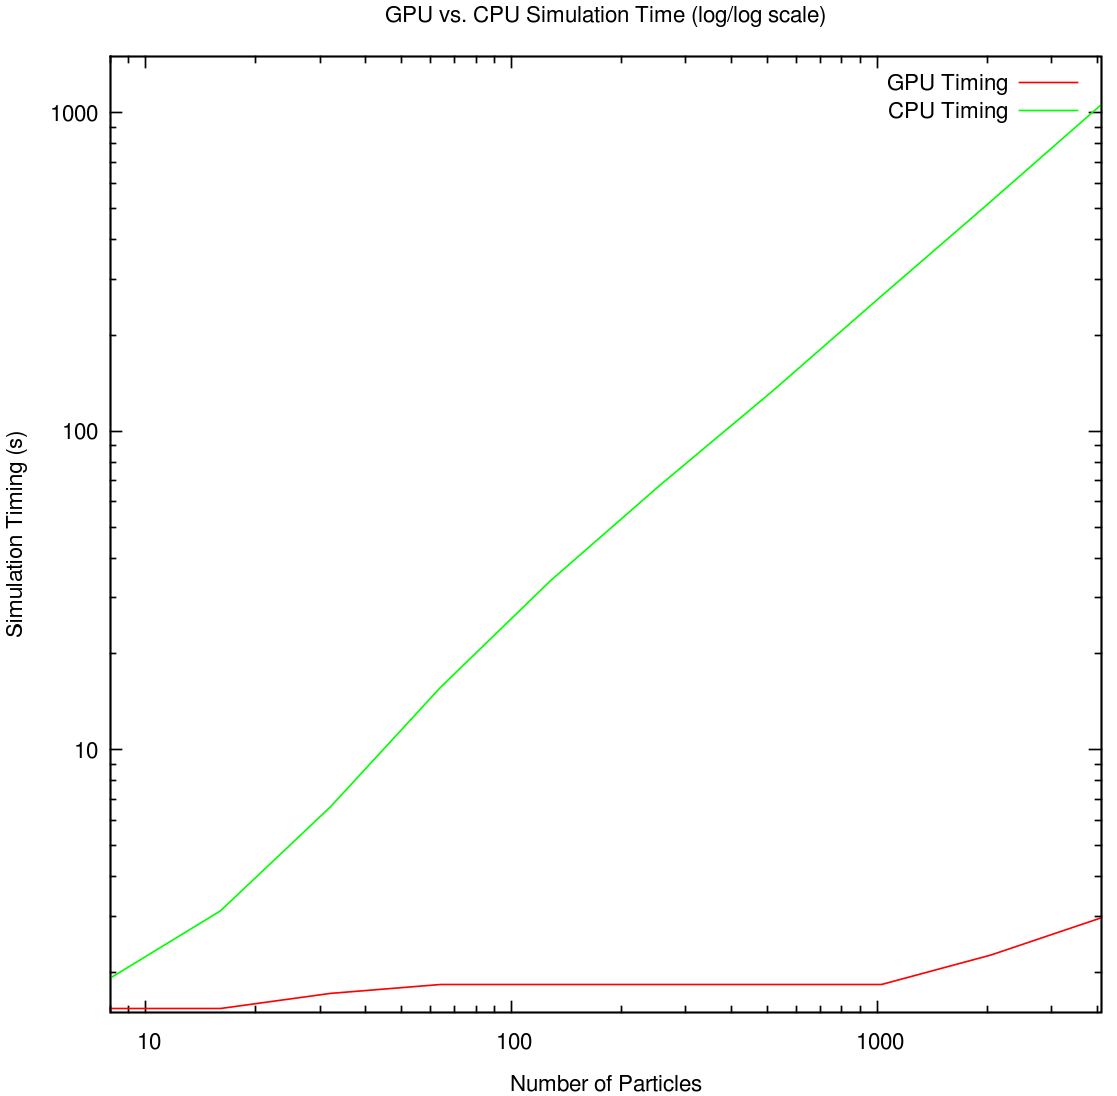
\includegraphics[width=\columnwidth]{figures/gpu_cpu_timings.png}
\caption{\label{fig:gpu-cpu-performance}The running time required as a
  function of the number of trajectories calculated using both the CPU
  and GPU simulators.  The plots have been placed on a log-log scale.
  The CPU simulator exhibits exactly the type of linear performance
  curve we expect, while GPU performance slowed by less than a factor
  of $2$ between $8$ and $4096$ trajectories.}
\end{figure}